Neural networks are trained under loss functions. So, for this purpose, we will compare the MSE loss, L1 loss, and Tukey's Biweight loss.

During the analysis, let $r_t = y_t - \hat{y}_t$ is residual for single output and let $\rho(.)$ corresponds to error for given residual. The loss of individual residuals are as follows:

\begin{eqnarray}
\rho(r_t) & = & \frac{1}{2} r_t^2 \label{eq:mse}\\
\rho(r_t) & = & \left|r_t\right| \label{eq:l1}\\
\rho(r_t) & = & \left\{\begin{array}{ll}{\frac{c^{2}}{6}\left[1-\left(1-\left(\frac{r_{i}}{c}\right)^{2}\right)^{3} \right]} & {, \text { if }\left|r_{i}\right| \leq c} \\ {\frac{c^{2}}{6}} & {, \text { if }\left|r_{t}\right|>c}\end{array}\right. \label{eq:tukey}
\end{eqnarray}

Where Equation \ref{eq:mse} corresponds to MSE loss, Equation \ref{eq:l1} refers to L1 loss and Equation \ref{eq:tukey} corresponds to Tukey's biweight loss functions. The results and figures of these losses are shown in the Figure \ref{fig:loss}.

\begin{figure}
    \centering
    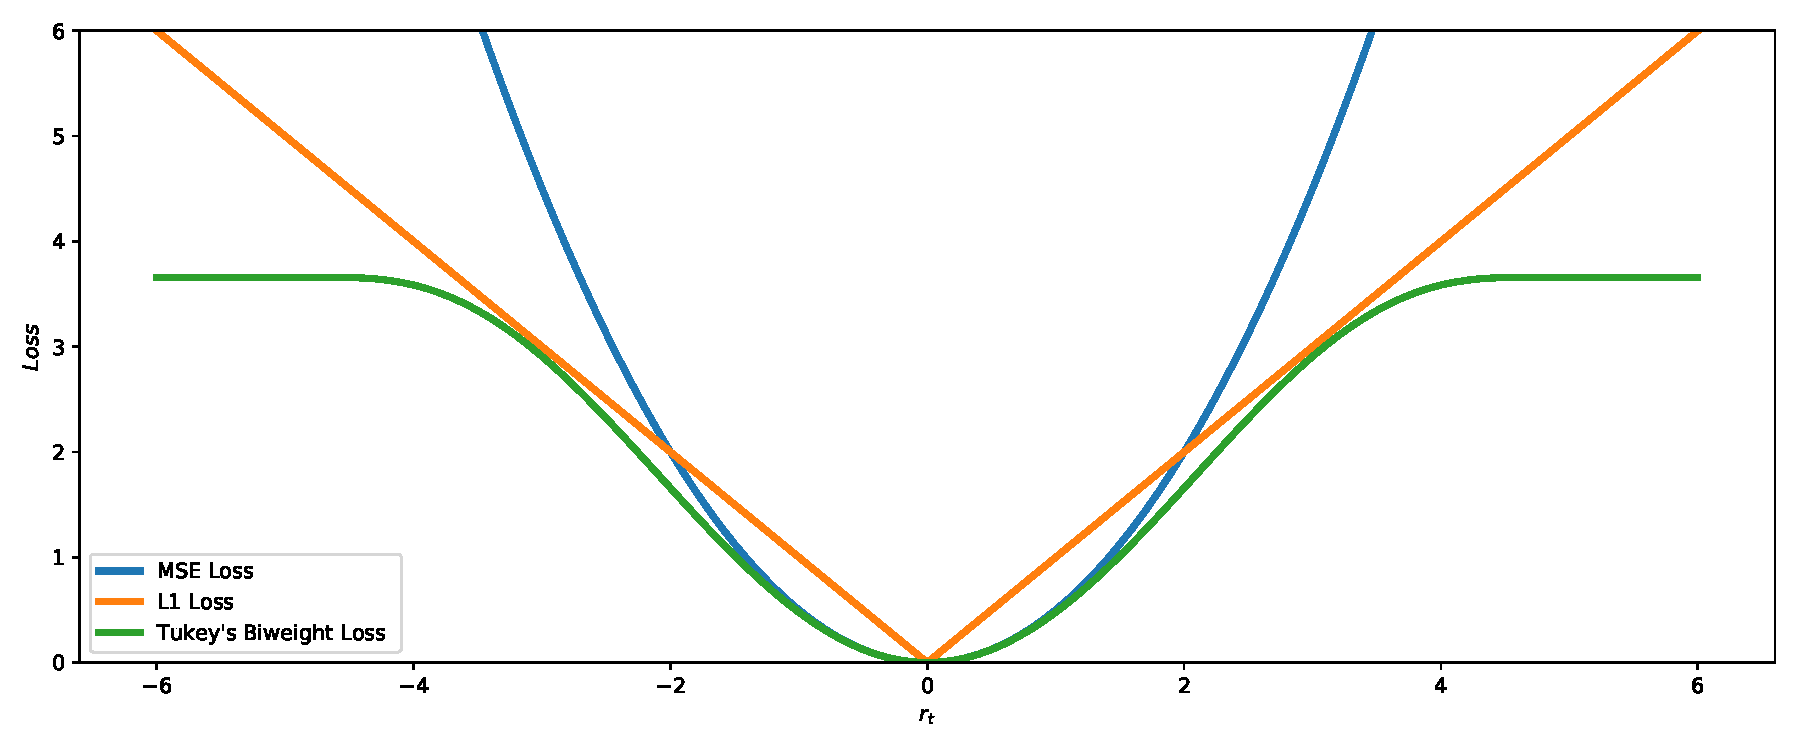
\includegraphics[width=0.9\textwidth]{figures/loss.pdf}
    \caption{Comparison of the loss functions}
    \label{fig:loss}
\end{figure}

The gradients of these loss functions are shown in Figure \ref{fig:gradient}.
Mathematically, these gradients are as follows, respectively:

\begin{eqnarray}
\rho^{\prime}(r_t) & = & r_t \label{eq:mse-derivative}\\
\rho^{\prime}(r_t) & = & \left\{\begin{array}{ll}{-1} & {, \text { if }\left|r_{t}\right|<0} \\ {1} & {, \text { if }\left|r_{t}\right|>0}\end{array}\right. \label{eq:l1-derivative}\\
\rho^{\prime}(r_t) & = & \left\{\begin{array}{ll}{r_{i}\left(1-\left(\frac{r_{t}}{c}\right)^{2}\right)^{2}} & {, \text { if }\left|r_{t}\right| \leq c} \\ {0} & {, \text { if }\left|r_{t}\right|>c}\end{array}\right. \label{eq:tukey-derivative}
\end{eqnarray}

\begin{figure}
    \centering
    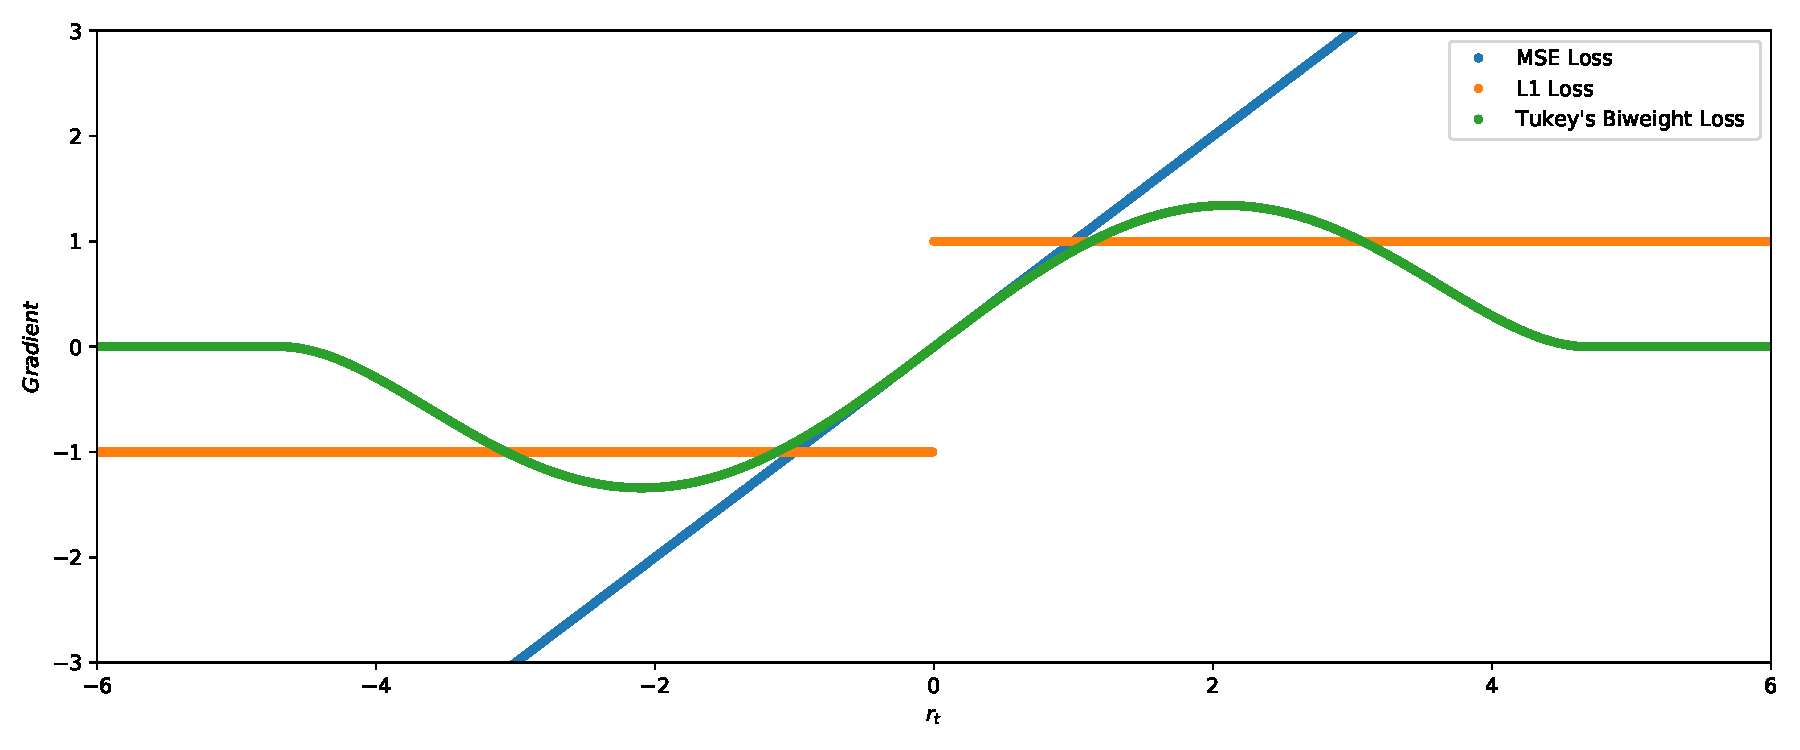
\includegraphics[width=0.9\textwidth]{figures/gradient.pdf}
    \caption{Comparison of the gradients of loss functions}
    \label{fig:gradient}
\end{figure}

The choice of $c$ of the `Tukey's biweight' loss depends on the `asymptotic efficiency'. Practically it sets to $4.685$, and it provides an asymptotic efficiency $95\%$ that of linear regression for the normal distribution. In the use case, one should calculate the {\it median absolute deviation} (MAD) of the residuals and set the new residuals as follows:

\begin{eqnarray}
    r_{t}^{\mathrm{MAD}} & =& \frac{r_t}{1.4826 \times \mathrm{MAD}_{t}}
\end{eqnarray}